\documentclass[tikz,border=4pt]{standalone}
\usepackage{xcolor}
\usetikzlibrary{arrows.meta,positioning,fit}
\definecolor{Navy}{RGB}{20,54,92}
\definecolor{Accent}{RGB}{184,63,49}
\begin{document}
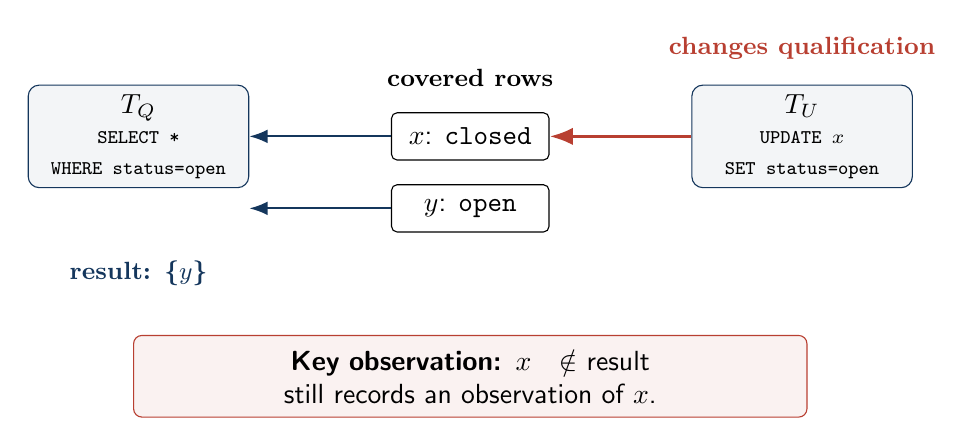
\begin{tikzpicture}[font=\sffamily, >=Latex,
  tx/.style={draw=Navy, rounded corners=4pt, fill=Navy!5, minimum width=28mm, minimum height=13mm, align=center},
  row/.style={draw, rounded corners=2pt, minimum width=20mm, minimum height=6mm, align=center}]
  \node[tx] (q) {\textbf{$T_Q$}\\[-1pt]\scriptsize \texttt{SELECT *}\\[-1pt]\scriptsize \texttt{WHERE status=open}};
  \node[row, right=18mm of q] (xold) {$x$: \texttt{closed}};
  \node[row, below=3mm of xold] (y) {$y$: \texttt{open}};
  \node[above=2mm of xold, font=\small\bfseries] {covered rows};
  \draw[-Latex, Navy, thick] (xold.west) -- (q.east |- xold.west);
  \draw[-Latex, Navy, thick] (y.west) -- (q.east |- y.west);
  \node[below=8mm of q, font=\small\bfseries, text=Navy] {result: \{$y$\}};
  \node[tx, right=18mm of xold] (u) {\textbf{$T_U$}\\[-1pt]\scriptsize \texttt{UPDATE $x$}\\[-1pt]\scriptsize \texttt{SET status=open}};
  \draw[-Latex, Accent, very thick] (u.west) -- (xold.east);
  \node[above=2mm of u, text=Accent, font=\small\bfseries] {changes qualification};
  \node[draw=Accent, rounded corners=3pt, fill=Accent!7, below=13mm of y, text width=82mm, align=center, inner sep=5pt] {\textbf{Key observation:} $x\notin$ result still records an observation of $x$.};
\end{tikzpicture}
\end{document}
